%!TEX TS-program = Arara
% arara: pdflatex: { shell: true }

\documentclass[11pt]{mimosis}
% \PassOptionsToClass{14pt}{scrbook}
\usepackage{metalogo}

\usepackage{textcomp}
\usepackage{gensymb}

%%%%%%%%%%%%%%%%%%%%%%%%%%%%%%%%%%%%%%%%%%%%%%%%%%%%%%%%%%%%%%%%%%%%%%%%
% Some of my favorite personal adjustments
%%%%%%%%%%%%%%%%%%%%%%%%%%%%%%%%%%%%%%%%%%%%%%%%%%%%%%%%%%%%%%%%%%%%%%%%
%
% These are the adjustments that I consider necessary for typesetting
% a nice thesis. However, they are *not* included in the template, as
% I do not want to force you to use them.

% This ensures that I am able to typeset bold font in table while still aligning the numbers
% correctly.
\usepackage{etoolbox}

\usepackage[binary-units=true]{siunitx}
\DeclareSIUnit\px{px}

\sisetup{%
  detect-all           = true,
  detect-family        = true,
  detect-mode          = true,
  detect-shape         = true,
  detect-weight        = true,
  detect-inline-weight = math,
}

%%%%%%%%%%%%%%%%%%%%%%%%%%%%%%%%%%%%%%%%%%%%%%%%%%%%%%%%%%%%%%%%%%%%%%%%
% Hyperlinks & bookmarks
%%%%%%%%%%%%%%%%%%%%%%%%%%%%%%%%%%%%%%%%%%%%%%%%%%%%%%%%%%%%%%%%%%%%%%%%

\usepackage[%
  colorlinks = true,
  citecolor  = Black,
  linkcolor  = Black,
  urlcolor   = Black,
  ]{hyperref}

\usepackage{bookmark}


%%%%%%%%%%%%%%%%%%%%%%%%%%%%%%%%%%%%%%%%%%%%%%%%%%%%%%%%%%%%%%%%%%%%%%%%
% Bibliography
%%%%%%%%%%%%%%%%%%%%%%%%%%%%%%%%%%%%%%%%%%%%%%%%%%%%%%%%%%%%%%%%%%%%%%%%
%
% I like the bibliography to be extremely plain, showing only a numeric
% identifier and citing everything in simple brackets. The first names,
% if present, will be initialized. DOIs and URLs will be preserved.

\usepackage[%
  autocite     = plain,
  backend      = bibtex,
  doi          = true,
  url          = true,
  giveninits   = true,
  hyperref     = true,
  maxbibnames  = 99,
  maxcitenames = 99,
  sortcites    = true,
  style        = alphabetic,
  citestyle    = alphabetic,
  backref      = true,
  ]{biblatex}


%%%%%%%%%%%%%%%%%%%%%%%%%%%%%%%%%%%%%%%%%%%%%%%%%%%%%%%%%%%%%%%%%%%%%%%%
% Some adjustments to make the bibliography more clean
%%%%%%%%%%%%%%%%%%%%%%%%%%%%%%%%%%%%%%%%%%%%%%%%%%%%%%%%%%%%%%%%%%%%%%%%
%
% The subsequent commands do the following:
%  - Removing the month field from the bibliography
%  - Fixing the Oxford commma
%  - Suppress the "in" for journal articles
%  - Remove the parentheses of the year in an article
%  - Delimit volume and issue of an article by a colon ":" instead of
%    a dot ""
%  - Use commas to separate the location of publishers from their name
%  - Remove the abbreviation for technical reports
%  - Display the label of bibliographic entries without brackets in the
%    bibliography
%  - Ensure that DOIs are followed by a non-breakable space
%  - Use hair spaces between initials of authors
%  - Make the font size of citations smaller
%  - Fixing ordinal numbers (1st, 2nd, 3rd, and so) on by using
%    superscripts

% Remove the month field from the bibliography. It does not serve a good
% purpose, I guess. And often, it cannot be used because the journals
% have some crazy issue policies.
\AtEveryBibitem{\clearfield{month}}
\AtEveryCitekey{\clearfield{month}}

% Fixing the Oxford comma. Not sure whether this is the proper solution.
% More information is available under [1] and [2].
%
% [1] http://tex.stackexchange.com/questions/97712/biblatex-apa-style-is-missing-a-comma-in-the-references-why
% [2] http://tex.stackexchange.com/questions/44048/use-et-al-in-biblatex-custom-style
%
\AtBeginBibliography{%
  \renewcommand*{\finalnamedelim}{%
    \ifthenelse{\value{listcount} > 2}{%
      \addcomma
      \addspace
      \bibstring{and}%
    }{%
      \addspace
      \bibstring{and}%
    }
  }
}

% Suppress "in" for journal articles. This is unnecessary in my opinion
% because the journal title is typeset in italics anyway.
\renewbibmacro{in:}{%
  \ifentrytype{article}
  {%
  }%
  % else
  {%
    \printtext{\bibstring{in}\intitlepunct}%
  }%
}

% Remove the parentheses for the year in an article. This removes a lot
% of undesired parentheses in the bibliography, thereby improving the
% readability. Moreover, it makes the look of the bibliography more
% consistent.
\renewbibmacro*{issue+date}{%
  \setunit{\addcomma\space}
    \iffieldundef{issue}
      {\usebibmacro{date}}
      {\printfield{issue}%
       \setunit*{\addspace}%
       \usebibmacro{date}}%
  \newunit}

% Delimit the volume and the number of an article by a colon instead of
% by a dot, which I consider to be more readable.
\renewbibmacro*{volume+number+eid}{%
  \printfield{volume}%
  \setunit*{\addcolon}%
  \printfield{number}%
  \setunit{\addcomma\space}%
  \printfield{eid}%
}

% Do not use a colon for the publisher location. Instead, connect
% publisher, location, and date via commas.
\renewbibmacro*{publisher+location+date}{%
  \printlist{publisher}%
  \setunit*{\addcomma\space}%
  \printlist{location}%
  \setunit*{\addcomma\space}%
  \usebibmacro{date}%
  \newunit%
}

% Ditto for other entry types.
\renewbibmacro*{organization+location+date}{%
  \printlist{location}%
  \setunit*{\addcomma\space}%
  \printlist{organization}%
  \setunit*{\addcomma\space}%
  \usebibmacro{date}%
  \newunit%
}

% Do not abbreviate "technical report".
\DefineBibliographyStrings{english}{%
  techreport = {technical report},
}

% Display the label of a bibliographic entry in bare style, without any
% brackets. I like this more than the default.
%
% Note that this is *really* the proper and official way of doing this.
\DeclareFieldFormat{labelnumberwidth}{#1\adddot}

% Ensure that DOIs are followed by a non-breakable space.
\DeclareFieldFormat{doi}{%
  \mkbibacro{DOI}\addcolon\addnbspace
    \ifhyperref
      {\href{http://dx.doi.org/#1}{\nolinkurl{#1}}}
      %
      {\nolinkurl{#1}}
}

% Use proper hair spaces between initials as suggested by Bringhurst and
% others.
\renewcommand*\bibinitdelim {\addnbthinspace}
\renewcommand*\bibnamedelima{\addnbthinspace}
\renewcommand*\bibnamedelimb{\addnbthinspace}
\renewcommand*\bibnamedelimi{\addnbthinspace}

% Make the font size of citations smaller. Depending on your selected
% font, you might not need this.
\renewcommand*{\citesetup}{%
  \biburlsetup
  \small
}

% \DeclareLanguageMapping{british}{bibliography-correct-ordinals}
% \DeclareLanguageMapping{english}{bibliography-correct-ordinals}
\bibliography{Thesis}

%%%%%%%%%%%%%%%%%%%%%%%%%%%%%%%%%%%%%%%%%%%%%%%%%%%%%%%%%%%%%%%%%%%%%%%%
% Fonts
%%%%%%%%%%%%%%%%%%%%%%%%%%%%%%%%%%%%%%%%%%%%%%%%%%%%%%%%%%%%%%%%%%%%%%%%

\ifxetexorluatex
  %\setmainfont{Minion Pro}
  \usepackage{microtype}
\else
  %\usepackage[osf,lining]{ebgaramond}  
  \usepackage[scale=0.7]{sourcecodepro}  
\fi






\usepackage{mathpazo}
\usepackage{lettrine}

\usepackage{makeidx}
\makeindex

% Enable urls in bibliography
\usepackage{url}

\newacronym[description={Principal component analysis}]{PCA}{PCA}{principal component analysis}
\newacronym                                            {SNF}{SNF}{Smith normal form}
\newacronym[description={Topological data analysis}]   {TDA}{TDA}{topological data analysis}

%\makeindex
\makeglossaries

%%%%%%%%%%%%%%%%%%%%%%%%%%%%%%%%%%%%%%%%%%%%%%%%%%%%%%%%%%%%%%%%%%%%%%%%
% Incipit
%%%%%%%%%%%%%%%%%%%%%%%%%%%%%%%%%%%%%%%%%%%%%%%%%%%%%%%%%%%%%%%%%%%%%%%%

\newcommand*{\titleGP}{\begingroup % Create the command for including the title page in the document
\centering % Center all text
\vspace*{\baselineskip} % White space at the top of the page

%\rule{\textwidth}{1.6pt}\vspace*{-\baselineskip}\vspace*{2pt} % Thick horizontal line
%\rule{\textwidth}{0.4pt}\\[1.0\baselineskip] % Thin horizontal line

{\huge Implementation and Didactical Visualization of the ChaCha Cipher Family in CrypTool 2}\\[0.2\baselineskip] % Title

%\rule{\textwidth}{0.4pt}\vspace*{-\baselineskip}\vspace{3.2pt} % Thin horizontal line
%\rule{\textwidth}{1.6pt}\\ % Thick horizontal line

\vspace*{\baselineskip}

{\Large Bachelor's Thesis\\[\baselineskip]} % Tagline(s) or further description
\vspace*{\baselineskip}

{\LARGE Ramdip Gill\\[\baselineskip]} % Editor list

\vspace*{\baselineskip} % Whitespace between location/year and editors

Supervisor\\
{\large  Priv.-Doz. Dr. Wolfgang Merkle\\[\baselineskip]} % Editor list

Second Supervisor\\
{\large  Prof. Dr. Frederik Armknecht\\[\baselineskip]} % Editor list

\vfil

Heidelberg,  \today \par % Location and year

\vspace*{\baselineskip}

{\itshape Faculty of Mathematics and Computer Science\par} % Editor affiliation
{\itshape Heidelberg University\par} % Editor affiliation

\endgroup}

 
\usepackage{mathtools}
\usepackage{amssymb}
\usepackage{siunitx}

\usepackage{blindtext}

% for code figures
\usepackage{minted}
\usepackage{listings}

% Corrects \autoref{}: chapter -> Chapter, section -> Section, subsection -> Section
\addto\extrasenglish{%
  \renewcommand{\chapterautorefname}{Chapter}%
  \renewcommand{\sectionautorefname}{Section}%
  \renewcommand{\subsectionautorefname}{Section}%
}

\includeonly{Sources/PluginImplementation}

\begin{document}

\frontmatter
\thispagestyle{empty}
  \titleGP  
  \cleardoublepage
  \pagestyle{empty}
  \begin{center}
  \textsc{Abstract}
\end{center}
%
\noindent \blindtext

\blindtext


  \begin{center}
  \textsc{Zusammenfassung}
\end{center}
%
\selectlanguage{ngerman}
\noindent \blindtext

\blindtext
\selectlanguage{english}
  % !TeX spellcheck = en_GB

\section*{Acknowledgment}

First of all, special thanks to Dr. Wolfgang Merkle who was willing to be the adviser from my home university, the University of Heidelberg. He introduced me to Prof. Dr. Frederik Armknecht from the University of Mannheim and thus laid the foundation for all of this. If not for Dr. Merkle, I don't know who else could have been the adviser for a bachelor's thesis in my preferred field, the field of cryptography. Most likely, I would have written my thesis in a different field.

\medskip
\noindent
I am also very grateful to Prof. Dr. Frederik Armknecht that he accepted me who he did not know at all beforehand. He offered me a wide variety of interesting subjects from which I could chose. In the end, I have chosen to develop a plug-in for \textit{CrypTool 2} (CT2), a open-source e-learning platform for cryptography and cryptanalysis.

\medskip
\noindent
Therefore, I want to extend my gratitude to the team behind CT2 whose support and welcomeness meant a lot to me. Prof. Bernhard Esslinger is the overall coordinator and Dr. Nils Kopal is the technical lead developer, both from the University of Siegen.
Whereas Prof. Dr. Armknecht gave me important feedback from a user's perspective since he uses CT2 in his lectures, Prof. Esslinger and Dr. Kopal always took their time to answer technical questions of mine. Additionally, Prof. Esslinger was always eager to remind me about things that were easy to miss like adding text to tooltips which I didn't even know existed. 

\medskip
\noindent
Finally, I also want to thank the people at my new employer Abusix, Inc. They made it possible for me to focus on my thesis by offering very flexible working hours. I am also very grateful that I could work on my thesis on their premises since going into the office was always a guarantee for a very productive day.
  % !TeX spellcheck = en_GB

\section*{Declaration of Authorship}

I hereby declare that the thesis submitted is my own unaided work. All direct or indirect sources used are acknowledged as references. The principles and recommendations \enquote{Verantwortung in der Wissenschaft} of Heidelberg University have been followed.
\vspace{5cm}\\
\noindent\rule[0.5ex]{8em}{0.5pt} \hfill \rule[0.5ex]{10em}{0.5pt}\\
\noindent first and last name \hfill city, date and signature
  \tableofcontents

\mainmatter
  \pagestyle{scrheadings}

  %%%%%%%%%%%%%%%%%%%%%%%%%%%%%%%%%%%%%%%%%%%%%%%%%%%%%%%%%%%%%%%%%%%%%%%%
\chapter{Introduction}

Applications of cryptology, the science behind creating encryptions (cryptography) and breaking them (cryptanalysis), date back far into ancient times. Around 3500 BC, the earliest known example of  cryptography was found which was a substitution cipher to conceal a formula for pottery glaze \cite{history}. Ever since, advancements in technology pushed the boundary for secure ciphers. Nowadays, in the Age of Information, the need for keeping sensitive information private is as important as ever before and will only get more important with widespread adoption of new technologies such as the Internet of Things. This is why research into new encryption standards has to continously take place.

The ChaCha cipher family by Daniel J. Bernstein is the result of such research. Because AES-GCM does not perform very well on devices without hardware acceleration such as wearable or mobile devices, Google has started to replace it in the TLS cipher suite of its browser Chrome with ChaCha20 for symmetric encryption and Poly1305 for authentication in 2014. Additionally, ChaCha is by design immune to previous TLS attacks such as padding-oracle or timing attacks and thus should improve security of HTTPS connections \cite{googlesecurityblog}.

This usage in TLS makes the ChaCha cipher family very attractive to include it in \textit{CrypTool 2 (CT2)}, a open-source e-learning platform for cryptography and cryptanalysis. It uses visual programming to teach cryptographic concepts and attacks.
  %%%%%%%%%%%%%%%%%%%%%%%%%%%%%%%%%%%%%%%%%%%%%%%%%%%%%%%%%%%%%%%%%%%%%%%%
\chapter{Related Work}
\label{sec:relatedWork}

This chapter discusses work relevant for the ChaCha plugin implementation and was therefore reviewed during the work on this thesis.

%%%%%%%%%%%%%%%%%%%%%%%%%%%%%%%%%%%%%%%%%%%%%%%%%%%%%%%%%%%%%%%%%%%%%%%%
\section{Salsa20 Cipher Family}
\label{sec:salsaCipher}

The ChaCha cipher family is based on the 256-bit stream cipher family Salsa20.

Salsa20/20, the 20 rounds variant, was developed by Daniel J. Bernstein in 2005 \cite{salsaspec} and submitted to eSTREAM, a European project to ``to promote the design of efficient and compact stream ciphers suitable for widespread adoption'' \cite{estream}.

It uses only add-rotate-XOR (ARX) operations for encryption which prevents timing attacks since they run in constant time on basically all platforms. Beside 256-bit keys, it also supports 128-bit keys. It internally uses a round function which transforms a 512-bit state, consisting of the key, four 32-bit constants, a 64-bit initialization vector and a 64-bit counter, into a keystream block. Since for the next keystream block, only the counter is incremented in the initial state, Salsa20 shares the same implementation advantages as block ciphers in counter mode, in particular the ability to generate output blocks in any order and in parallel \cite{salsaspec}.

Bernstein later introduced other variants with 8 and 12 rounds, named Salsa20/8 and Salsa20/12, to let users decide between a faster, but less secure cipher. Other round variants like 9, 10 or 11 were not introduced because the difference in speed would be insignificant \cite{salsa812}. The ChaCha cipher family received the same round variants. 

There is also a variant of Salsa20 called XSalsa20 which supports 192-bit initialization vectors. Since its implementation varies quite a bit from the Salsa20/r variants and Bernstein introduced XSalsa20 as part of a new cipher family (based on Salsa20), this cipher is of no relevance for this thesis \cite{xsalsa20spec}. There is a XChaCha20 variant but it ``is currently not widely implemented outside the libsodium library [a software library for cryptography], due to the absence of formal specification'' \cite{xchacha20}.

The specification of Salsa20 is very relevant for ChaCha because the specification for ChaCha only mentions the differences \cite{chachaspec}. Therefore, to implement ChaCha, one has to read through the specification of Salsa20.  However, in Chapter \ref{chap:chacha}, I will go over the specification of ChaCha without assuming prior knowledge about Salsa20.

%%%%%%%%%%%%%%%%%%%%%%%%%%%%%%%%%%%%%%%%%%%%%%%%%%%%%%%%%%%%%%%%%%%%%%%%

\section{Salsa20 CrypTool 2 Plugin}
\label{sec:salsaCT2Plugin}

\begin{figure}
\label{fig:salsa.template}
\centering
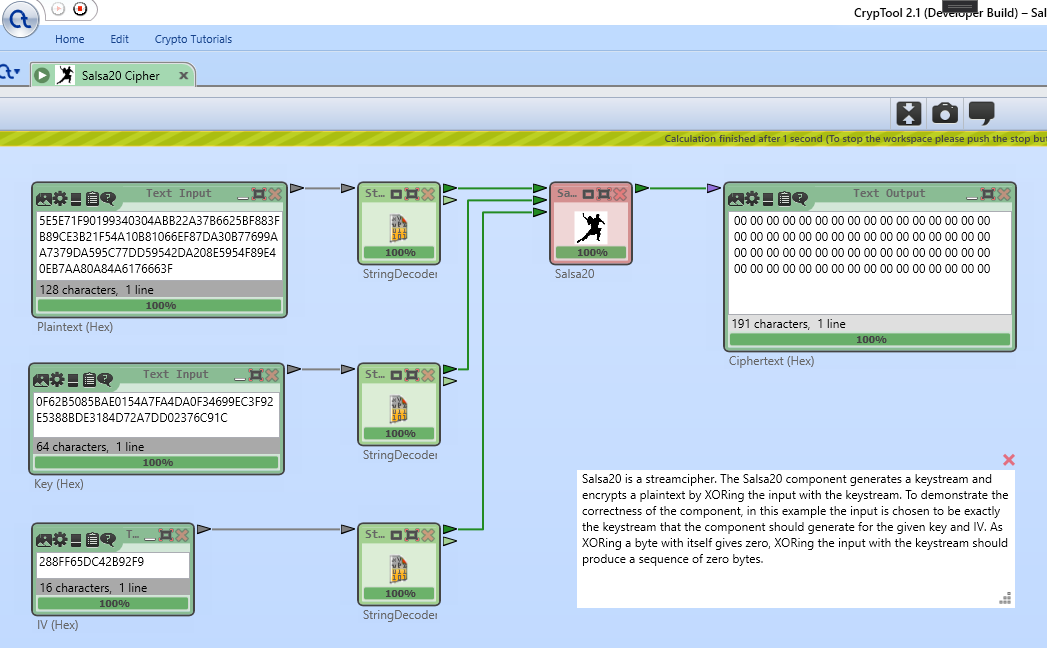
\includegraphics[width=\textwidth]{figures/ct2/salsa-crop.png}
\caption[Salsa20 CT2 template]{CT2 template for the already existing Salsa20 plugin}
\end{figure}

CrypTool 2 already has a plugin for the Salsa20 cipher but without a visualization.

During my work on the ChaCha visualization, I thought about how I could reuse my code for the ChaCha visualization to create a visualization for the Salsa20 cipher. I figured that it would not be as straight-forward as I assumed in the beginning since the visualization goes very into detail and thus the differences would involve at least different XAML code. For example, since the state is built up differently, the visualization about the state matrix initialization would need to be adapted. Also, the quarterround is slightly different which also needs to be reflected in the visualization. 

Nonetheless, I think that most of the codebase used for the ChaCha cipher could be reused to create a Salsa20 visualization, especially the navigation system and how the intermediate results are stored and retrieved for visualization. I will further discuss this in Chapter \ref{chap:futureWork}.


%%%%%%%%%%%%%%%%%%%%%%%%%%%%%%%%%%%%%%%%%%%%%%%%%%%%%%%%%%%%%%%%%%%%%%%%
\section{Other CrypTool 2 Cipher Visualizations}
\label{sec:otherCT2CipherVisualizations}

In this section, I will discuss ideas that I got from existing CrypTool 2 cipher visualizations which were also created by students during their bachelor thesis.

\subsection{AES Visualization}
\label{sec:aesVisualization}

\begin{figure}
\label{fig:aes}
\centering
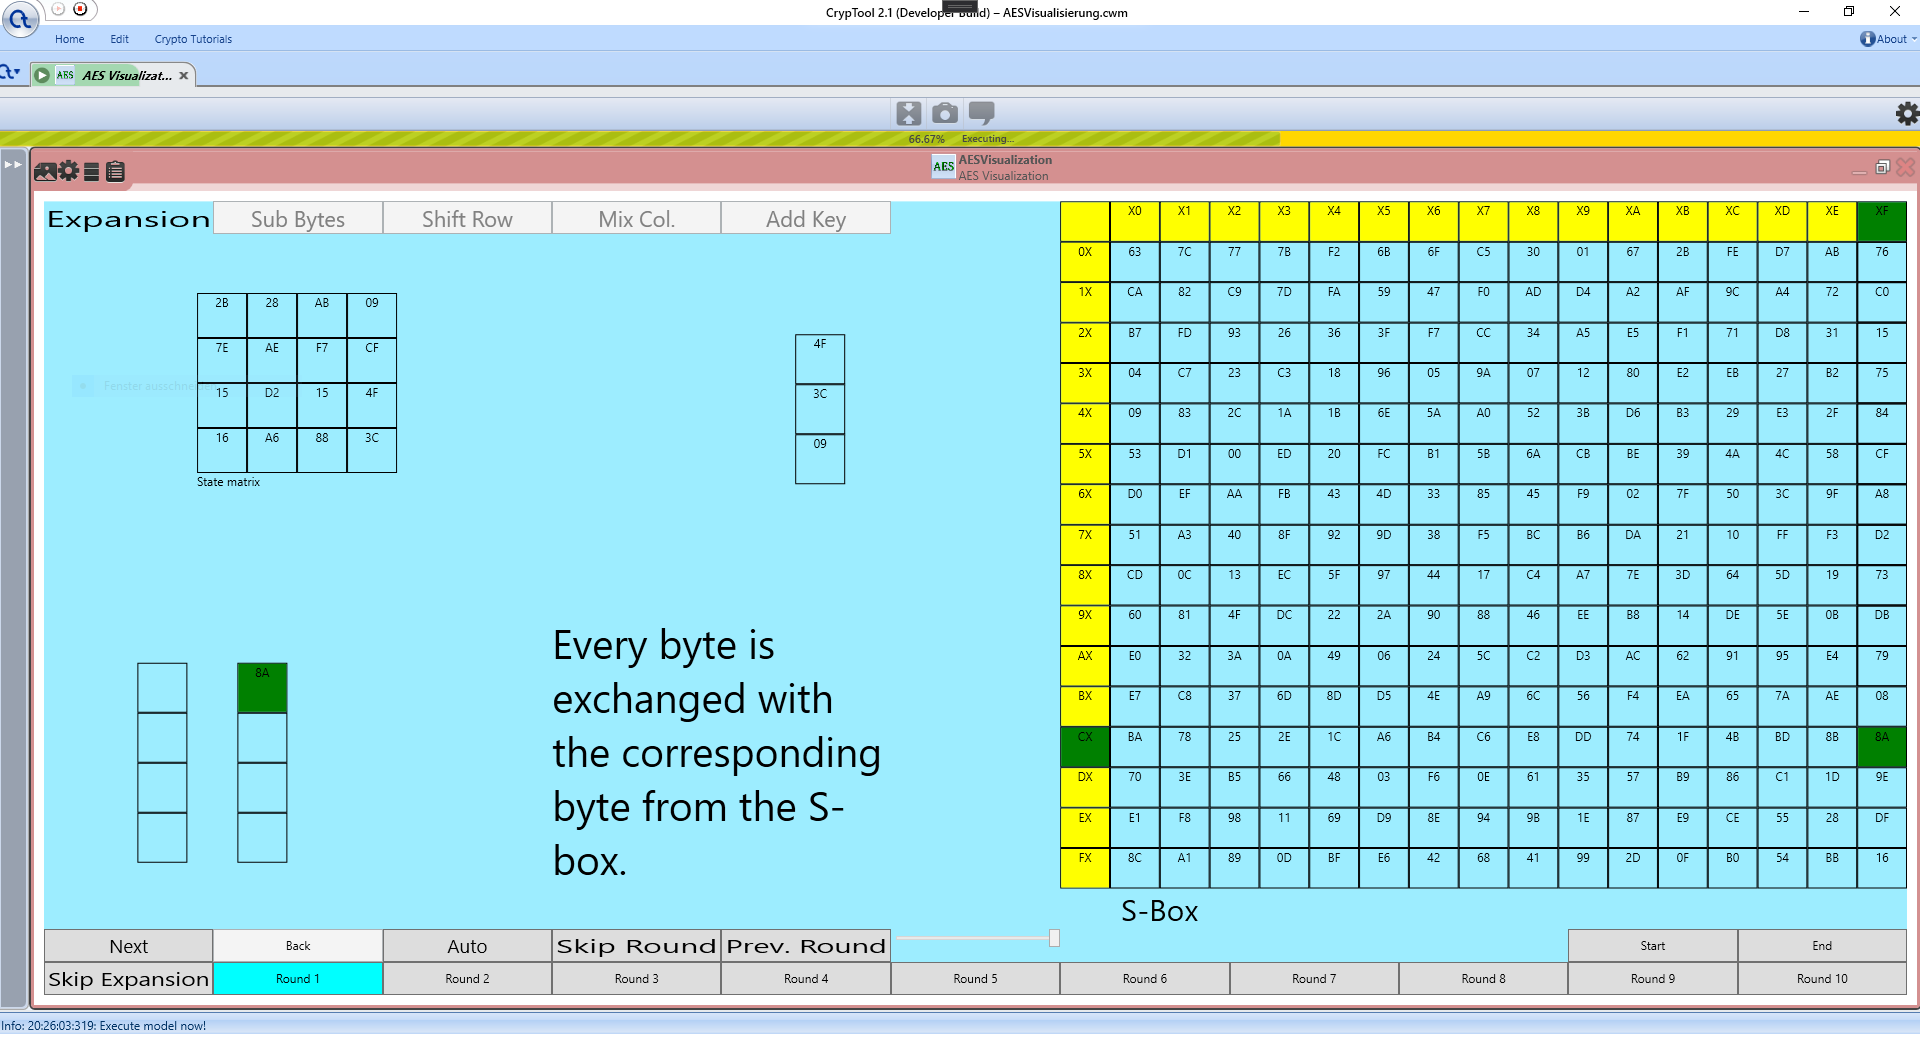
\includegraphics[width=\textwidth]{figures/ct2/aes.png}
\caption{AES visualization plugin}
\end{figure}

Matthias Becher created a visualization for the AES cipher during his bachelor thesis in 2016. It was the visualization of which I took the most inspiration for my own implementation. I also read through his bachelor thesis to see how he solved some of the problems that I encountered. For example, he wrote the following:

``The first big decision that had to be made was whether the states after each encryption operation would be calculated during the visualization or precalculated and stored at the start of the execution. One feature the plugin should have was to not only jump ahead to later operations but also to go back to previous ones. That means if the values were calculated during the visualization every time you went back they would have to be recalculated from the start. Therefore, I decided to precompute and store results of each operation in an array of byte arrays..'' \cite{aesthesis}

I came to the exact same conclusion that the values need to be precalculated for the reasons he mentioned.

Looking through his visualization, I liked how he changed the background of the elements to catch the user's attention. This is shown in Figure \ref{fig:aes}. I have used a similar mechanic during the ChaCha hash function visualization where I put a light blue background onto the state elements which will be used as the quarterround input. Also during the quarterround, I extensively used background coloring to tell the user where he should pay his attention.

Another thing I adopted from his visualization was the navigation in the top-left corner. I placed my page navigation there.

What I wanted to do differently in my navigation was to not show so many buttons all the time to the user. I was quite overwhelmed by all the buttons in the bottom navigation bar on the start even though they were disabled. Therefore, on pages which have no actions, I had no buttons in the bottom row. On pages with actions, a simple slider with a previous and next button did suffice. For the ChaCha hash function, which needed additional navigation, my navigation bar looked similar but still felt in my opinion less crowded, especially because I did not use buttons for every single round but a text input .

Further, I was confused why I could not use the ``Back'' button during the ``Expansion'' or ``Encryption'' step. For my plugin, I wanted to let the user navigate to any step in the visualization fairly simple. To achieve this, I needed to make sure that the user knows where he is and where he needs to click to go to a particular step. To give the user the information he needed, I used the dedicated page navigation in the top-left corner which stays the same on every page and tells the user on which page he currently is with bold font. Further, I numbered every single action on each page together with an action text input and how many actions a page has. The text input makes it possible for the user to immediately jump to an action.

\subsection{DES Visualization}
\label{sec:desVisualization}

\begin{figure}
\label{fig:des}
\centering
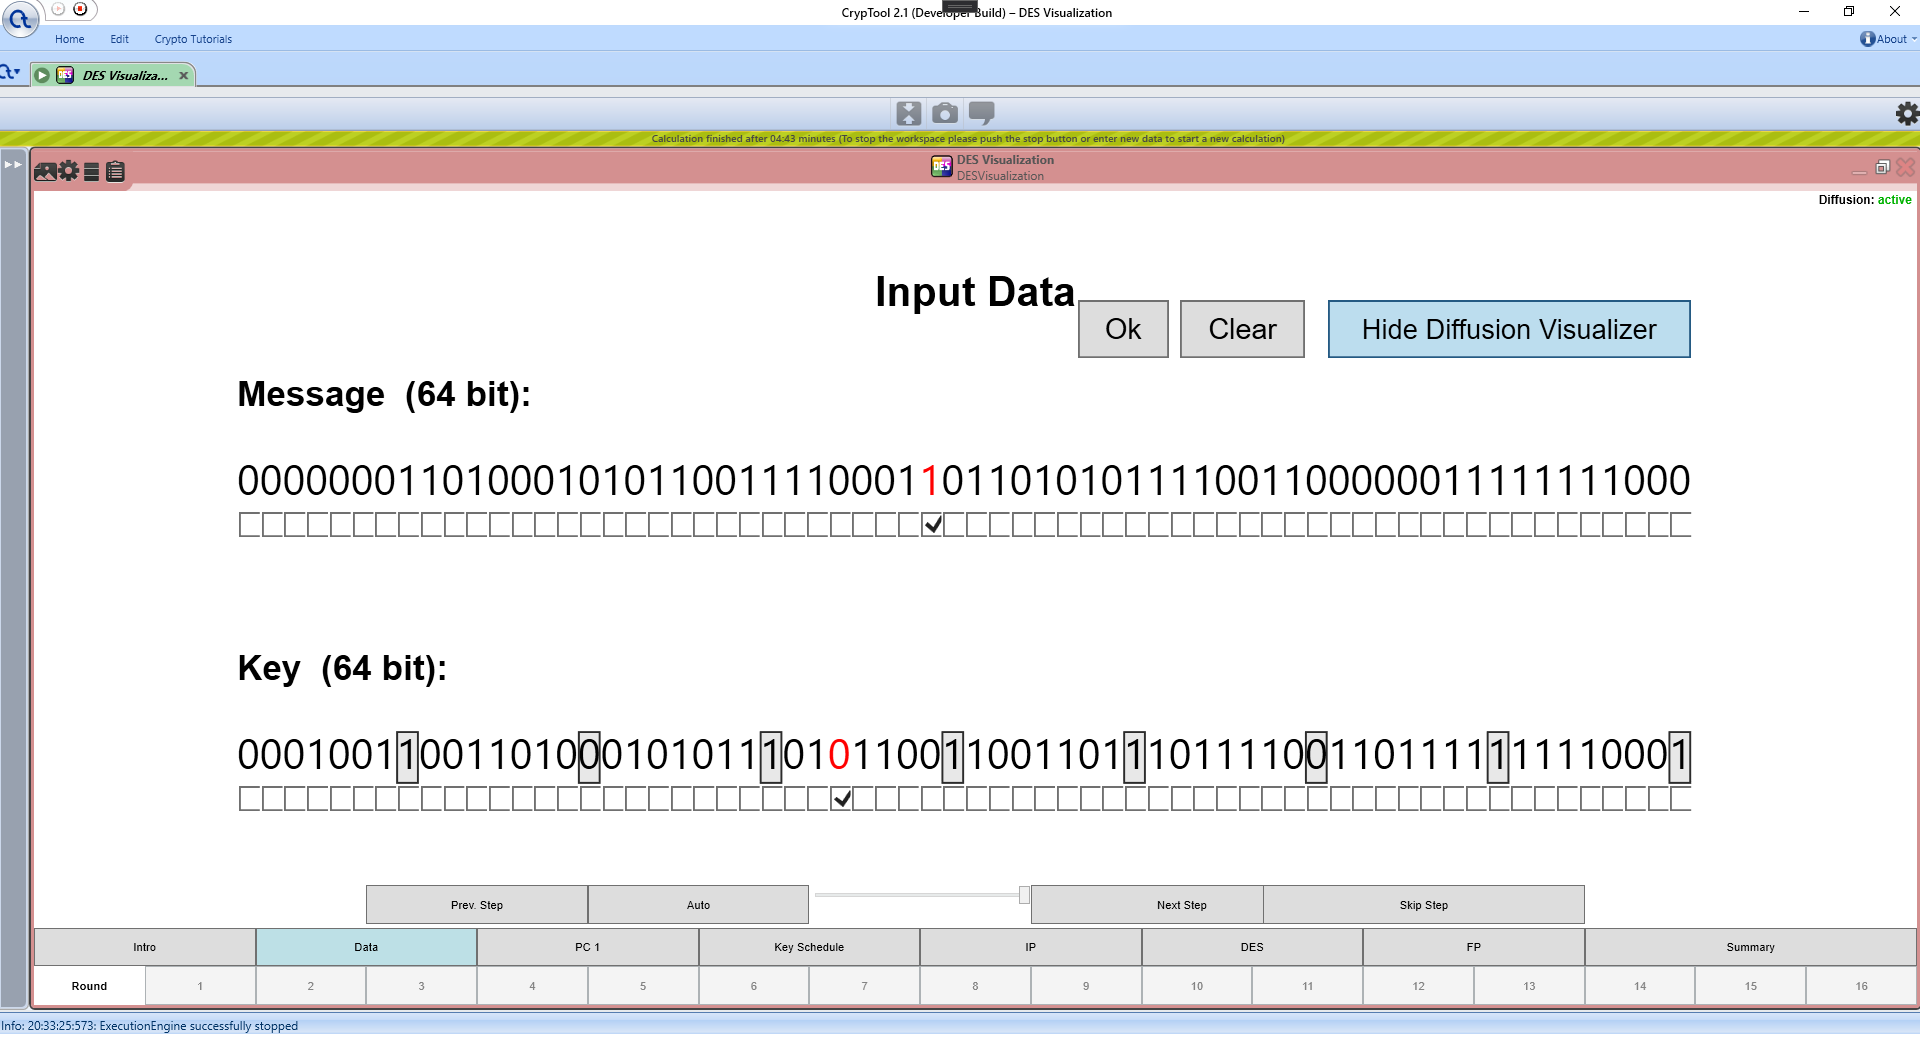
\includegraphics[width=\textwidth]{figures/ct2/des.png}
\caption{DES visualization plugin}
\end{figure}

The DES visualization was also created by a student, Lars Hoffman, for his bachelor thesis. His approach to visualizing the diffusion had the most influence on my diffusion visualization. In Figure \ref{fig:des}, you can see the page on which the user can flip bits to activate diffusion. The message and key with flipped bits will then be used to show the diffusion property of DES. 

Throughout the visualization, all values are shown in binary. This makes it possible to just mark flipped bits red since if a bit is marked red, we immediately know the value of the diffusion run (we just flip the red bit). 

I used the same coloring approach but noticed that since the ChaCha cipher was using longer keys and 512-bit blocks compared to the 64-bit blocks of DES, I needed to use hex strings for my values to save canvas space. This lead to a loss of information about the value of the diffusion run if only marking red the hexadecimal characters which are different. Therefore, I combined the usage of red color together with showing both values in two rows. In the row for the diffusion value, the difference is still marked red for easier visual recognition. This is shown in Figure \ref{fig:chachahash.mid.qr.with.diffusion}.

\subsection{Avalanche Visualization}
\label{sec:avalancheVisualization}



  % !TeX spellcheck = en_GB

%%%%%%%%%%%%%%%%%%%%%%%%%%%%%%%%%%%%%%%%%%%%%%%%%%%%%%%%%%%%%%%%%%%%%%%%
\chapter{ChaCha Specification}
\label{chap:chacha}

To help with understanding the plug-in visualization and for the sake of completeness, I will summarize the specification of the ChaCha cipher in this chapter.

ChaCha is a 256-bit stream cipher based on Salsa20, both developed by Daniel J. Bernstein. It was designed to improve diffusion per round while maintaining or even increasing the performance compared to Salsa20. This makes it more secure than Salsa20 with the same amount of rounds. It was developed in the year 2008, 3 years after Salsa20 \cite{chachaspec}.

The specification can be broken apart into five main points: \\
The \textit{quarter-round} function, the \textit{little-endian} function, a hash function which utilizes the two other mentioned functions, the setup of the 512-bit state and finally, the encryption/decryption process, bringing all the individual pieces together.

I will start with the quarter round function.

\section{Quarter-round Function}
\label{sec:chacha.qr}

The ChaCha quarter-round function takes in four 32-bit unsigned integers which we will name $a$, $b$, $c$ and $d$. It also returns four 32-bit unsigned integers.\\
It modifies its input values as described in the following pseudo-code:

\begin{center}
\begin{minipage}{0.5\linewidth}
\texttt{quarterround(a,b,c,d):} \\
\hspace*{2em}\texttt{a += b; d  \^{}= a; d} \verb|<<<|\texttt{= 16} \\
\hspace*{2em}\texttt{c += d; b \^{}= c; b} \verb|<<<|\texttt{= 12} \\
\hspace*{2em}\texttt{a += b; d \^{}= a; d} \verb|<<<|\texttt{= 8} \\
\hspace*{2em}\texttt{c += d; b \^{}= c; b} \verb|<<<|\texttt{= 7} \\
\hspace*{2em}\texttt{return a, b, c, d}
\end{minipage}
\end{center}

I will call one row, consisting of one 32-bit addition, one XOR and one shift operation, a \textit{quarter-round step}. This naming convention will be reused in Section \ref{sec:userInterface}.

\section{Little-Endian Function}
\label{sec:chacha.littleendian}

The little-endian function takes in one 32-bit unsigned integer and reverses its byte order; also returning a 32-bit unsigned integer.  \\
It can be implemented as follows:

\begin{center}
\begin{minipage}{0.8\linewidth}
\texttt{littleendian(x):} \\
\hspace*{2em}\texttt{x0 = (x} \verb|>>|\texttt{ 24) \& 0xff} \\
\hspace*{2em}\texttt{x1 = (x} \verb|>>|\texttt{ 16) \& 0xff} \\
\hspace*{2em}\texttt{x2 = (x} \verb|>>|\texttt{ 8) \& 0xff} \\
\hspace*{2em}\texttt{x3 = x \& 0xff} \\
\hspace*{2em}\texttt{return (x3 } \verb|<<|\texttt{ 24) | (x2 }\verb|<<|\texttt{ 16) | (x1 }\verb|<<|\texttt{ 8) | x0}
\end{minipage}
\end{center}

\begin{remark}
Its naming has nothing to do with system endianness, but was just named like this by Bernstein for unknown reasons (most likely because reversing the byte order is what needs to be done when transmitting data between systems of different endianness).
\end{remark}

\section{ChaCha Hash Function}
\label{sec:chacha.hash}

The ChaCha hash function takes in 16 32-bit unsigned integers and returns 16 32-bit unsigned integers. The input vector $(y_0, y_1, y_2, \dots, y_{15})$ can be written as a 4$\times$4 matrix:

\begin{equation*}
\begin{pmatrix}
y_0 & y_1 & y_2 & y_3 \\
y_4 & y_5 & y_6 & y_7 \\
y_8 & y_9 & y_{10} & y_{11} \\
y_{12} & y_{13} & y_{14} & y_{15}\\
\end{pmatrix}
\end{equation*}

Using this matrix representation helps with understanding why Bernstein calls some rounds \textit{column rounds} and others \textit{diagonal rounds} in his paper (one round consists of four quarter-rounds): \\
The ChaCha hash function first iterates through all columns and then through all diagonals of the matrix; applying the quarter-round function to the four entries of each column/diagonal. After the first four quarter-rounds it therefore has changed all columns of the matrix. This is what Bernstein calls a column round in his paper. After the next four quarter-rounds, it changed all diagonals of the matrix which Bernstein analogously calls a diagonal round.

To summarize, the following quarter-rounds make up one column round:
\begin{center}
\begin{minipage}{0.5\linewidth}
\texttt{quarterround($y_0$, $y_4$, $y_8$, $y_{12}$)} \\
\texttt{quarterround($y_1$, $y_5$, $y_9$, $y_{13}$)} \\
\texttt{quarterround($y_2$, $y_6$, $y_{10}$, $y_{14}$)} \\
\texttt{quarterround($y_3$, $y_7$, $y_{11}$, $y_{15}$)} \\
\end{minipage}
\end{center}
\noindent whereas the following quarterrounds make up one diagonal round:
\begin{center}
\begin{minipage}{0.5\linewidth}
\texttt{quarterround($y_0$, $y_5$, $y_{10}$, $y_{15}$)} \\
\texttt{quarterround($y_1$, $y_6$, $y_{11}$, $y_{12}$)} \\
\texttt{quarterround($y_2$, $y_7$, $y_8$, $y_{13}$)} \\
\texttt{quarterround($y_3$, $y_4$, $y_9$, $y_{14}$)} \\
\end{minipage}
\end{center}

After a set amount of rounds (8, 12, or 20), the input vector is added to the vector on which the rounds were run. Then the byte order of each matrix entry is reversed using the little-endian function.

Having explained the basic structure of the ChaCha hash function, the following pseudo-code should complete the readers comprehension of it:

\begin{center}
\begin{minipage}{\linewidth}
\texttt{chachahash(y):} \\
\hspace*{2em}\texttt{z = copy(y)}\\
\hspace*{2em}\texttt{for(i = 0; i < ROUNDS; i += 2) \{}\\
\hspace*{4em}\texttt{// column round}\\
\hspace*{4em}\texttt{y[0], y[4], y[8], y[12] = quarterround(y[0], y[4], y[8], y[12])}\\
\hspace*{4em}\texttt{y[1], y[5], y[9], y[13] = quarterround(y[1], y[5], y[9], y[13])}\\
\hspace*{4em}\texttt{y[2], y[6], y[10], y[14] = quarterround(y[2], y[6], y[10], y[14])}\\
\hspace*{4em}\texttt{y[3], y[7], y[11], y[15] = quarterround(y[3], y[7], y[11], y[15])}\\
\hspace*{4em}\texttt{// diagonal round}\\
\hspace*{4em}\texttt{y[0], y[5], y[10], y[15] = quarterround(y[0], y[5], y[10], y[15])}\\
\hspace*{4em}\texttt{y[1], y[6], y[11], y[12] = quarterround(y[0], y[5], y[10], y[15])}\\
\hspace*{4em}\texttt{y[2], y[7], y[8], y[13] = quarterround(y[0], y[5], y[10], y[15])}\\
\hspace*{4em}\texttt{y[3], y[4], y[9], y[14] = quarterround(y[0], y[5], y[10], y[15])}\\
\hspace*{2em}\texttt{\}}\\
\hspace*{2em}\texttt{for(i = 0; i < 16; i += 1) \{}\\
\hspace*{4em}\texttt{y[i] += z[i]}\\
\hspace*{4em}\texttt{y[i] = littleendian(y[i])}\\
\hspace*{2em}\texttt{\}}\\
\hspace*{2em}\texttt{return y}
\end{minipage}
\end{center}

\section{ChaCha State Matrix}
\label{sec:chacha.matrix}

ChaCha internally uses a 512-bit state for keystream generation. The ChaCha hash function modifies this state to generate a keystream block. \\
In this section, I will explain how the state is setup which is then passed in 32-bit blocks to the ChaCha hash function.

The state is made up of a 128-bit constant, a 256-bit key section and a 128-bit nonce section. To demonstrate that the author had no hidden intent with picking his constants (nothing-up-my-sleeve number), he defined the constants to be ``expand 16-byte k'' for 128-bit keys and ``expand 32-byte k'' for 256-bit keys in ASCII.

In the 128-bit key variant, the key is concatenated with itself to create a 256-bit key. This concatenated key is then used for the state setup. If the key is already 256-bit, we do nothing and just use it as it is for the state setup.

The nonce section, which consists of a block counter and the initialization vector, is where the original version and the IETF version differ. In the original version, a 64-bit counter and a 64-bit initialization vector is used whereas the IETF version is using a 32-bit counter and a 96-bit initialization vector. \\
This means that the IETF version only partitions the nonce differently. Their reasoning to have a longer initialization vector was that with a 32-bit counter, one can encrypt messages up to 256GiB which should be enough and therefore one could make use of a bigger initialization vector. Since we need to make sure that a initialization vector is never reused with the same key, we can use a bigger initialization vector to make it more secure in cases where the same key is used by multiple senders. This is done by partitioning the 96-bit word into one 32-bit and one 64-bit section. The 32-bit section could be a unique value per sender and the last 64 bits could be a counter which is incremented for every message \cite{rfc8439}.

All state parameters are encoded by first splitting them into 32-bit chunks whose byte order is reversed except for the counter, whose byte order is first completely reversed and afterwards split into 32-bit chunks. Their 32-bit blocks are then ordered as follows to form the 512-bit state matrix:

\begin{equation*}
\begin{pmatrix}
\texttt{CONSTANT}& \texttt{CONSTANT} & \texttt{CONSTANT} & \texttt{CONSTANT} \\
\texttt{KEY} & \texttt{KEY} & \texttt{KEY} & \texttt{KEY} \\
\texttt{KEY} & \texttt{KEY} & \texttt{KEY} & \texttt{KEY} \\
\texttt{COUNTER} & \texttt{COUNTER/IV} & \texttt{IV} & \texttt{IV} \\
\end{pmatrix}
\end{equation*}

Example (all numbers are in hexadecimal with \texttt{:} as separation between bytes and already split into 32-bit chunks):\\

\begin{tabular}{ l l }
 \texttt{key (256-bit)} & \texttt{01:02:03:04 05:06:07:08 09:0a:0b:0c 0d:0e:0f:10} \\ 
 & \texttt{11:12:13:14 15:16:17:18 19:1a:1b:1c 1d:1e:1f:20}\\
 \texttt{IV} & \texttt{00:11:22:33 44:55:66:77} \\  
\texttt{Counter} & \texttt{00:00:00:00 00:00:00:01} \\
\end{tabular}
\\

\noindent Since we used a 256-bit key, we will use the ASCII constants ``expand 32-byte k''. Their byte representation is:\\

\begin{tabular}{ l l }
\texttt{Constants\phantom{MMMM}} & \texttt{65:78:70:61 6e:64:20:33 32:2d:62:79 74:65:20:6b} \\
\end{tabular}
\\

\noindent The resulting state matrix:

\begin{equation*}
\begin{pmatrix}
\texttt{61:70:78:65}& \texttt{33:20:64:6e} & \texttt{79:62:2d:32} & \texttt{6b:20:65:74} \\
\texttt{04:03:02:01} & \texttt{08:07:06:05} & \texttt{0c:0b:0a:09} & \texttt{10:0f:0e:0d} \\
\texttt{14:13:12:11} & \texttt{18:17:16:15} & \texttt{1c:1b:1a:19} & \texttt{20:1f:1e:1d} \\
\texttt{00:00:00:01} & \texttt{00:00:00:00} & \texttt{33:22:11:00} & \texttt{77:66:55:44} \\
\end{pmatrix}
\end{equation*}

\section{Encryption/Decryption}
\label{sec:chacha.encryption}

To encrypt or decrypt a input text, it is XOR'ed with the keystream. \\
To generate the keystream, the ChaCha hash function is continuously used to create 512-bit keystream blocks until we have enough to XOR every byte of the input text. The input to the ChaCha hash function is the 512-bit initial state as explained in the previous section. After each keystream block, the counter is incremented to have a different initial state as the input each time.

Since we are operating on streams, if the input message is not a multiple of 512-bit, the bits of the last block of the input message are left-aligned and the remaining bits of the keystream are dropped. This means that the output will always be the exact same length as the input.

There is no difference between encryption or decryption because XOR is the inverse to itself.

  %%%%%%%%%%%%%%%%%%%%%%%%%%%%%%%%%%%%%%%%%%%%%%%%%%%%%%%%%%%%%%%%%%%%%%%%
\chapter{Plugin Implementation}
\label{chap:PluginImplementation}

\blindtext[1]

%%%%%%%%%%%%%%%%%%%%%%%%%%%%%%%%%%%%%%%%%%%%%%%%%%%%%%%%%%%%%%%%%%%%%%%%
\section{Goals}
\label{sec:goals}

\blindtext[2]

%%%%%%%%%%%%%%%%%%%%%%%%%%%%%%%%%%%%%%%%%%%%%%%%%%%%%%%%%%%%%%%%%%%%%%%%
\section{Implementation details}
\label{sec:implementationDetails}

\blindtext[1]

%%%%%%%%%%%%%%%%%%%%%%%%%%%%%%%%%%%%%%%%%%%%%%%%%%%%%%%%%%%%%%%%%%%%%%%%

\subsection{Key Features}
\label{sec:keyFeatures}

\blindtext[2]

\subsection{User Interface}
\label{sec:userInterface}

\blindtext[8]

\subsection{Architecture}
\label{sec:Architecture}

\blindtext[8]

%%%%%%%%%%%%%%%%%%%%%%%%%%%%%%%%%%%%%%%%%%%%%%%%%%%%%%%%%%%%%%%%%%%%%%%%

\section{Encountered Problems}
\label{sec:encounteredProblems}

In this section, I will discuss the main problems I encountered during implementation. To briefly summarize, they mainly consisted of how to create a simple, intuitive user interface and how the system behind the interface should be designed to have the best or at least a reasonable performance. \\ In the other visualizations, I noticed that I was quite overwhelmed by the amount of buttons which were visible, even though not always enabled. So I wanted to keep my user interface as simple as possible while not restricting the user in his ability to navigate through the visualization. \\ Regarding the performance, I have read in the thesis about the AES visualization that to create a fluent user experience where he can navigate back and forth between all steps, the intermediate values need to be calculated beforehand and saved since we don't want to stop at each step to calculate the next value or recalculate everything from the start if the user wants to go backwards.\\
I hope that the description of these problems and the solutions I have found may help future students in writing their own plugins.

\subsection{Performance}

The peformance of the plugin was essentially coupled to how the navigation system was designed. Other things like the calculation of the intermediate values for the visualization were unsignificant because they are created by the ChaCha cipher anyway and must just be saved somewhere to not lose them. I realized this relationship early in development when I had my first page with many page actions on it and wanted to skip ahead a lot of actions. While implementing this feature which would enable the user to skip from any action to any other action, I realized that when skipping more than 100 actions, it already took about 750ms during which the UI was unresponsive. As can be seen in FIGURE X, this time increased linearly so it was quite clear that I needed to do something about this, especially because the page with the most actions had over 3000 single actions.

\par

The root cause of the problem was the navigation system design which I called in hindsight \textbf{\textit{linear navigation system}}. It consisted of defining actions which build upon each other. This means that if we are at action 1 and want to go to action 5, we need to execute all the code inside the action definitions between 1 and 5 to arrive at the page state as it should be at action 5. \\
I came up with this design to have a smooth implementation experience where I only have to write the actual page state changes between two actions instead of duplicating a lot of code since the page state changes which were applied during a previous page were most of the times still visible when moving to the next action. This complements how the user experiences the visualization because the actions are numbered in a sequence and thus are inherently linear. Thus it made a lot of sense to me to reflect this in the system architecture.
\par
Since this "design flaw" was not the leading cause of the performance problem (going through a for-loop of size 3000 does not directly lead to performance issues), I want to briefly explain how the actual action implementation looked like. In Figure \ref{code.linear}, you can see sample code.

\begin{figure}
\caption{Sample for action definition in the linear navigation system}
\label{code.linear}
\begin{minted}[frame=single, breaklines]{csharp}
PageAction constantsStepDescriptionAction = new PageAction(() =>
{
	string desc = "The 512-bit (128-byte) ChaCha state can be interpreted as a 4x4 matrix, where each entry consists of 4 bytes interpreted as little-endian. The first 16 bytes consist of the constants. ";
	pres.Nav.AddBold(pres.UIStateMatrixStepDescription, desc);
}, pres.Nav.Undo);
PageAction constantsInputAction = new PageAction(() =>
{
	pres.Nav.UnboldLast(pres.UIStateMatrixStepDescription);
	pres.Nav.Replace(pres.UITransformInput, pres.HexConstants);
}, pres.Nav.Undo);
\end{minted}
\end{figure}
  %%%%%%%%%%%%%%%%%%%%%%%%%%%%%%%%%%%%%%%%%%%%%%%%%%%%%%%%%%%%%%%%%%%%%%%%
\chapter{Future Work}
\label{chap:futureWork}

In this chapter, I will describe how the plugin could be further improved to make it more useful for the audience of CrypTool 2.

\begin{description}[style=nextline]
\item[Diffusion: XOR input and button to toggle between XOR and actual values] 

Adding a third input to the Diffusion page where the user can explicitly set the XOR of the primary and secondary value would better fit the needs of cryptanalysist who want to study the diffusion property of the cipher since one is more interested in the difference between two values than in their actual values. For example, if we just want to flip one bit, we could just type in a single 1 anywhere into the XOR input. \\
Using the same argument, a button with which one toggle between seeing the XOR of the intermediate values and their actual values during visualization would be useful.

\item[Diffusion: Better overview over flipped bits at the end of each round]

In the Avalanche visualization, at the end of the visualization, I have seen that the author provided a overview over the percentage of flipped bits at the end of each round. I found this very sensible because it shows how the amount of flipped bits goes very fast up to around 50\% and then stays near it which is one would expect from a secure cipher. \\
I have thought about using a plot instead of the simple text which is updated at the end of each round but due to canvas and time constraints, I did not further pursue this idea. I could image to integrate such an overview directly into the Diffusion page. This would need cipher execution while still on the page instead on page exit but this would not be a big problem since a button to start cipher execution would suffice.

\pagebreak

\item[Automatic navigation]

As mentioned in Section \ref{sec:aesVisualization}, in the AES visualization, I have seen a button which lets the visualization run without further user interaction needed. A slider was provided to adjust the speed. I think that such a button could be useful for the ChaCha visualization, too, especially for the page about the ChaCha hash function with its many actions. \\
Since I am already using asynchronous navigation for the action slider (which I think would be needed to let a timer run without blocking the UI), I think implementing this feature could easily be integrated within the existing navigation system. Only page switches could maybe get tricky since the action navigation is handled within each page thus navigating out of a page may not be straight-forward. I have noticed that the automatic navigation in the AES visualization does stop between each step so switching the page automatically may not even be desired.

\item[Salsa20 visualization]

As mentioned in Section \ref{sec:salsaCT2Plugin}, using the now existing codebase for ChaCha visualization to create a Salsa20 visualization would definitely increase the value gained from this thesis. This would at least need adaption of the XAML code for the state matrix initialization and the quarterround since ChaCha and Salsa20 differ in this aspects from each other. It would most likely even increase the value of the ChaCha visualization, since both ciphers could then be compared side-by-side. Since the visualizations would be very similar, comparing them and their diffusion property should be very easy.

\item[Localization and online help]

Currently, most texts are only localized in English. Only the memofields, component labels and plaintext value are also available in German. This should be changed in the near future. Further, there should be an online help for the ChaCha plugin which opens by selecting it and pressing F1.

\end{description}

%%%%%%%%%%%%%%%%%%%%%%%%%%%%%%%%%%%%%%%%%%%%%%%%%%%%%%%%%%%%%%%%%%%%%%%%

% This ensures that the subsequent sections are being included as root
% items in the bookmark structure of your PDF reader.
\bookmarksetup{startatroot} 
\backmatter

  % \begingroup 
  %   \let\clearpage\relax 
  %   \glsaddall
  %   \printglossary
  % \endgroup

  \label{sec:index}
  
  \printbibliography
  
\end{document}